%%%%%%%%%%%%%%%%%%%%%%%%%%%%%%%%%%%%%%%%%%%%%%%
%
% Template per Elaborato di Laurea
% DISI - Dipartimento di Ingegneria e Scienza dell’Informazione
%
% update 2015-09-10
%
% Per la generazione corretta del 
% pdflatex nome_file.tex
% bibtex nome_file.aux
% pdflatex nome_file.tex
% pdflatex nome_file.tex
%
%%%%%%%%%%%%%%%%%%%%%%%%%%%%%%%%%%%%%%%%%%%%%%%

% formato FRONTE RETRO
\documentclass[epsfig,a4paper,11pt,titlepage,twoside,openany]{book}
\usepackage{epsfig}
\usepackage{plain}
\usepackage{setspace}
\usepackage{listings} % For code
\usepackage[paperheight=29.7cm,paperwidth=21cm,outer=1.5cm,inner=2.5cm,top=2cm,bottom=2cm]{geometry} % per definizione layout
\usepackage{titlesec} % per formato custom dei titoli dei capitoli
\usepackage[hidelinks]{hyperref} % for a clickable table of contents
%%%%%%%%%%%%%%
% supporto lettere accentate
%
%\usepackage[latin1]{inputenc} % per Windows;
\usepackage[utf8x]{inputenc} % per Linux (richiede il pacchetto unicode);
%\usepackage[applemac]{inputenc} % per Mac.

\usepackage[dvipsnames]{xcolor}

\singlespacing

\usepackage[italian]{babel}

\definecolor{verylightgray}{rgb}{.97,.97,.97}

\lstdefinelanguage{Solidity}{
	keywords=[1]{anonymous, assembly, assert, balance, break, call, callcode, case, catch, class, constant, continue, constructor, contract, debugger, default, delegatecall, delete, do, else, emit, event, experimental, export, external, false, finally, for, function, gas, if, implements, import, in, indexed, instanceof, interface, internal, is, length, library, log0, log1, log2, log3, log4, memory, modifier, new, payable, pragma, private, protected, public, pure, push, require, return, returns, revert, selfdestruct, send, solidity, storage, struct, suicide, super, switch, then, this, throw, transfer, true, try, typeof, using, value, view, while, with, addmod, ecrecover, keccak256, mulmod, ripemd160, sha256, sha3}, % generic keywords including crypto operations
	keywordstyle=[1]\color{blue}\bfseries,
	keywords=[2]{address, bool, byte, bytes, bytes1, bytes2, bytes3, bytes4, bytes5, bytes6, bytes7, bytes8, bytes9, bytes10, bytes11, bytes12, bytes13, bytes14, bytes15, bytes16, bytes17, bytes18, bytes19, bytes20, bytes21, bytes22, bytes23, bytes24, bytes25, bytes26, bytes27, bytes28, bytes29, bytes30, bytes31, bytes32, enum, int, int8, int16, int24, int32, int40, int48, int56, int64, int72, int80, int88, int96, int104, int112, int120, int128, int136, int144, int152, int160, int168, int176, int184, int192, int200, int208, int216, int224, int232, int240, int248, int256, string, uint, uint8, uint16, uint24, uint32, uint40, uint48, uint56, uint64, uint72, uint80, uint88, uint96, uint104, uint112, uint120, uint128, uint136, uint144, uint152, uint160, uint168, uint176, uint184, uint192, uint200, uint208, uint216, uint224, uint232, uint240, uint248, uint256, var, void, ether, finney, szabo, wei, days, hours, minutes, seconds, weeks, years},	% types; money and time units
	keywordstyle=[2]\color{teal}\bfseries,
	keywords=[3]{block, blockhash, coinbase, difficulty, gaslimit, number, timestamp, msg, data, gas, sender, sig, value, now, tx, gasprice, origin, mapping},	% environment variables
	keywordstyle=[3]\color{violet}\bfseries,
	identifierstyle=\color{black},
	sensitive=true,
	comment=[l]{//},
	morecomment=[s]{/*}{*/},
	commentstyle=\color{gray}\ttfamily,
	stringstyle=\color{red}\ttfamily,
	morestring=[b]',
	morestring=[b]"
}

\lstset{
	language=Solidity,
    extendedchars=true,
    backgroundcolor=\color{verylightgray},
	basicstyle=\footnotesize\ttfamily,
	showstringspaces=false,
	showspaces=false,
	tabsize=3,
	breaklines=true,
	showtabs=false,
	captionpos=b
}
\lstdefinelanguage{JavaScript}{
    keywords={break, case, catch, continue, debugger, default, delete, do, else, finally, for, function, if, in, instanceof, new, return, switch, this, throw, try, typeof, var, void, while, with, const, await, async},
    morecomment=[l]{//},
    morecomment=[s]{/*}{*/},
    morestring=[b]',
    morestring=[b]",
    sensitive=true
}

\begin{document}

  % nessuna numerazione
  \pagenumbering{gobble}
  \pagestyle{plain}

\thispagestyle{empty}

\begin{center}
  \begin{figure}[h!]
    \centerline{
\psfig{file=img/logo_unitn_black_center.eps,width=0.6\textwidth}}
  \end{figure}

  \vspace{2 cm} 

  \LARGE{Dipartimento di Ingegneria e Scienza dell’Informazione\\}

  \vspace{1 cm} 
  \Large{Corso di Laurea in\\
    Informatica
    %Ingegneria dell'Informazione e delle Comunicazioni
    %Ingegneria dell'Informazione e Organizzazione d'Impresa
    %Ingegneria Elettronica e delle Telecomunicazioni
  }

  \vspace{2 cm} 
  \Large\textsc{Elaborato finale\\} 
  \vspace{1 cm} 
  \Huge\textsc{La gestione di ruoli e permessi sulla blockchain Ethereum\\}
  \Large{\it{}}


  \vspace{2 cm} 
  \begin{tabular*}{\textwidth}{ c @{\extracolsep{\fill}} c }
  \Large{Supervisore} & \Large{Laureando}\\
  \Large{Prof. Alberto Montresor}& \Large{Matteo Golinelli}\\
  \end{tabular*}

  \vspace{2 cm} 

  \Large{Anno accademico 2018/2019}
  
\end{center}



  %\clearpage

%%%%%%%%%%%%%%%%%%%%%%%%%%%%%%%%%%%%%%%%%%%%%%%%%%%%%%%%%%%%%%%%%%%%%%%%%%
%%%%%%%%%%%%%%%%%%%%%%%%%%%%%%%%%%%%%%%%%%%%%%%%%%%%%%%%%%%%%%%%%%%%%%%%%%
%% Nota
%%%%%%%%%%%%%%%%%%%%%%%%%%%%%%%%%%%%%%%%%%%%%%%%%%%%%%%%%%%%%%%%%%%%%%%%%%
%% Sezione Ringraziamenti opzionale
%%%%%%%%%%%%%%%%%%%%%%%%%%%%%%%%%%%%%%%%%%%%%%%%%%%%%%%%%%%%%%%%%%%%%%%%%%
%%%%%%%%%%%%%%%%%%%%%%%%%%%%%%%%%%%%%%%%%%%%%%%%%%%%%%%%%%%%%%%%%%%%%%%%%%
  %\input{ringraziamenti}
  %\clearpage
  \pagestyle{plain} % nessuna intestazione e pie pagina con numero al centro

  
  % inizio numerazione pagine in numeri arabi
  \mainmatter

%%%%%%%%%%%%%%%%%%%%%%%%%%%%%%%%%%%%%%%%%%%%%%%%%%%%%%%%%%%%%%%%%%%%%%%%%%
%%%%%%%%%%%%%%%%%%%%%%%%%%%%%%%%%%%%%%%%%%%%%%%%%%%%%%%%%%%%%%%%%%%%%%%%%%
%% Nota
%%%%%%%%%%%%%%%%%%%%%%%%%%%%%%%%%%%%%%%%%%%%%%%%%%%%%%%%%%%%%%%%%%%%%%%%%%
%% Si ricorda che il numero massimo di facciate e' 30.
%% Nel conteggio delle facciate sono incluse 
%%   indice
%%   sommario
%%   capitoli
%% Dal conteggio delle facciate sono escluse
%%   frontespizio
%%   ringraziamenti
%%   allegati    
%%%%%%%%%%%%%%%%%%%%%%%%%%%%%%%%%%%%%%%%%%%%%%%%%%%%%%%%%%%%%%%%%%%%%%%%%%
%%%%%%%%%%%%%%%%%%%%%%%%%%%%%%%%%%%%%%%%%%%%%%%%%%%%%%%%%%%%%%%%%%%%%%%%%%

    % indice
    \tableofcontents
    \clearpage
    
    % gruppo per definizone di successione capitoli senza interruzione di pagina
    \begingroup
      % nessuna interruzione di pagina tra capitoli
      % ridefinizione dei comandi di clear pagei
      \renewcommand{\cleardoublepage}{} 
      \renewcommand{\clearpage}{} 
      % redefinizione del formato del titolo del capitolo
      % da formato
      %   Capitolo X
      %   Titolo capitolo
      % a formato
      %   X   Titolo capitolo
      
      \titleformat{\chapter}
        {\normalfont\Huge\bfseries}{\thechapter}{1em}{}
        
      \titlespacing*{\chapter}{0pt}{0.59in}{0.02in}
      \titlespacing*{\section}{0pt}{0.20in}{0.02in}
      \titlespacing*{\subsection}{0pt}{0.10in}{0.02in}
      
      % sommario
      \chapter*{Sommario} % senza numerazione
\label{sommario}

\addcontentsline{toc}{chapter}{Sommario} % da aggiungere comunque all'indice

Questa tesi di laurea tratta dell'esperienza di tirocinio svolta nell'arco di tempo intercorso tra febbraio e giugno del 2019 presso l'azienda Digicando.

La contraffazione causa ogni anno la perdita di svariati miliardi di euro in diversi settori produttivi e di posti di lavoro. La produzione di merci contraffatte è un fenomeno in aumento. La vendita di merci contraffatte, oltre a comportare una perdita economica per i produttori autentici, comporta un danno d'immagine per gli stessi, data la scarsa qualità dei prodotti contraffatti ma ritenuti originali dagli acquirenti. Quando si acquista un prodotto non è infatti generalmente possibile verificarne l'autenticità e la qualità. Le recensioni giocano un ruolo fondamentale nella scelta di un prodotto, ma non è possibile verificarne la genuinità. Per i produttori è inoltre difficile vigilare sulla catena logistica ed sul lavoro dei venditori.

L'azienda Digicando offre un servizio che mira a risolvere i problemi sopraelencati. Attualmente il sistema è sviluppato con un'architettura client-server centralizzata, ma l'azienda ha avviato lo sviluppo del suo servizio basato sulle tecnologie della blockchain Ethereum. L'obiettivo di questa transizione è fornire un servizio trasparente che mantenga una cronologia immodificabile dei trasferimenti di un prodotto nella catena di distribuzione, aperto al controllo di chiunque.

L'implementazione su blockchain del servizio di Digicando, pur essendo in uno stato avanzato dello sviluppo, risulta limitato da alcune mancanze, prima fra tutte l'impossibilità di gestire le azioni riservate a Digicando o ad un produttore da più indirizzi Ethereum ed i permessi ad essi associati. Si è quindi reso necessario lo sviluppo di un sistema di gestione dei ruoli e dei permessi orientato agli indirizzi.

Il sistema di gestione dei ruoli è stato sviluppato nel linguaggio di programmazione Solidity, proprio della blockchain Ethereum, e comprende due contratti. Il primo contratto funge da registro ed è destinato alla semplice memorizzazione dei ruoli associati a dei determinati indirizzi. Il secondo contratto fornisce una funzione che permette di verificare la validità di strutture gerarchiche complesse.

Il sistema sviluppato soddisfa i requisiti definiti dall'azienda ed una volta integrato con l'implementazione presente ha permesso di risolvere il problema descritto precedentemente. I contratti di Digicando e dei produttori sono ora gestibili da più indirizzi ed è possibile rimuoverne o aggiungerne altri.
      \newpage
%%%%%%%%%%%%%%%%%%%%%%%%%%%%%%%%%%%%%%%%%%%%%%%%%%%%%%%%%%%%%%%%%%%%%%%%%%
%%%%%%%%%%%%%%%%%%%%%%%%%%%%%%%%%%%%%%%%%%%%%%%%%%%%%%%%%%%%%%%%%%%%%%%%%%
%% Nota
%%%%%%%%%%%%%%%%%%%%%%%%%%%%%%%%%%%%%%%%%%%%%%%%%%%%%%%%%%%%%%%%%%%%%%%%%%
%% Sommario e' un breve riassunto del lavoro svolto dove si descrive 
%% l’obiettivo, l’oggetto della tesi, le metodologie e 
%% le tecniche usate, i dati elaborati e la spiegazione delle conclusioni 
%% alle quali siete arrivati.
%% Il sommario dell’elaborato consiste al massimo di 3 pagine e deve contenere le seguenti informazioni: 
%%   contesto e motivazioni
%%   breve riassunto del problema affrontato
%%   tecniche utilizzate e/o sviluppate
%%   risultati raggiunti, sottolineando il contributo personale del laureando/a
%%%%%%%%%%%%%%%%%%%%%%%%%%%%%%%%%%%%%%%%%%%%%%%%%%%%%%%%%%%%%%%%%%%%%%%%%%
%%%%%%%%%%%%%%%%%%%%%%%%%%%%%%%%%%%%%%%%%%%%%%%%%%%%%%%%%%%%%%%%%%%%%%%%%%      
      
      %%%%%%%%%%%%%%%%%%%%%%%%%%%%%%%%
      % lista dei capitoli
      %
      %
      % NOTA: perchè il documento compili senza errori
      % i capitoli devono essere preceduti da una linea
      % completamente vuota

      \chapter{La tecnologia Blockchain}
\label{cha:tecnologia-blockchain}
La blockchain è una tecnologia relativamente nuova, infatti è stata creata nel 2008. Ha come obiettivo primario il mantenimento di un registro (o libro mastro) immodificabile, al quale è possibile solo aggiungere nuove informazioni.

\section{Definizioni}
\label{definizioni}
Per meglio comprendere questo capitolo è opportuno definire i termini più utilizzati:
\begin{itemize}
    \item \emph{Sistema distribuito}: un sistema distribuito è un sistema composto da computer indipendenti, connessi utilizzando un \emph{middleware}. I computer che partecipano al sistema condividono le loro risorse e capacità per fornire una rete integrata e coerente agli utenti \cite{distribuito}. Queste macchine hanno uno stato condiviso, operano simultaneamente e possono fallire individualmente senza influire sullo stato della rete \cite{distribuito-medium}.
    \item \emph{Sistema decentralizzato}: un sistema decentralizzato è un sistema dove non c'è un singolo punto dove vengono prese le decisioni. Ogni nodo prende una decisione sul proprio comportamento singolarmente ed il comportamento risultante del sistema è l'aggregazione dei singoli comportamenti \cite{decentralizzato}.
    \item \emph{Peer-to-peer}: è un'architettura nella quale ogni computer è sia \emph{client} che \emph{server} verso gli altri partecipanti \cite{p2p}.
\end{itemize}

\section{Storia}
L'idea di utilizzare una catena di blocchi protetti crittograficamente viene descritta nel 1991 da Stuart Haber e W. Scott Stornetta, con l'obiettivo di implementare un sistema di \emph{timestamping} di documenti immodificabile. Nel 1992 viene introdotto dagli stessi studiosi l'utilizzo di alberi Merkle per permettere la certificazione di più documenti in un unico blocco. Un albero Merkle è una particolare struttura ad albero che permette una verifica efficiente e sicura di grandi strutture dati \cite{merkle-tree}.

Questo studio è stato utilizzato come base da Satoshi Nakamoto, pseudonimo di una persona o un gruppo di persone, per concettualizzare la prima blockchain nel 2008 attraverso un \emph{paper}. Nakamoto ha migliorato in modo sostanziale il sistema introducendo l'utilizzo dell'algoritmo \emph{Proof of Work} (spiegato nella Sezione \ref{proof-of-work}), che regola l'aggiunta dei blocchi alla catena senza la necessità di una firma di una parte fidata. Negli anni successivi questo progetto è stato implementato da Nakamoto ed utilizzato come componente principale della criptovaluta \emph{Bitcoin} \cite{blockchain}.
Negli ultimi anni sono nate molte criptovalute basate sulla tecnologia blockchain (descritte nella Sezione \ref{criptovalute}). Oggi è possibile acquistare beni e servizi di vario genere con le criptovalute. Spesso, a causa della loro potenziale anonimità, sono utilizzate nei mercati neri per l'acquisto e lo scambio di beni e servizi illegali.

\section{Blockchain}
\label{blockchain}
Una \emph{Blockchain} è un registro crescente di \emph{record}, chiamati blocchi, connessi tra loro utilizzando la crittografia. Questo registro è condiviso da tutte le parti che operano all'interno di una rete distribuita di computer. Ogni blocco contiene un hash crittografico del blocco precedente, un timestamp e dei dati riguardanti delle transazioni. Una blockchain non è modificabile per definizione, in quanto ogni modifica invaliderebbe l'intera struttura.

Una blockchain è composta da:
\begin{itemize}
    \item Una \emph{rete peer-to-peer} che connette i partecipanti e propaga le transazioni ed i blocchi di transazioni verificate mediante un protocollo di \emph{gossip} standardizzato.
    \item Messaggi, sotto forma di \emph{transazioni}, che rappresentano le transizioni dello stato.
    \item Un insieme di \emph{regole di consenso}, che stabiliscono le caratteristiche di una transazione valida e di una transizione di stato valida.
    \item Una \emph{macchina a stati} che processa le transazioni in accordo con le regole del consenso.
    \item Una \emph{catena di blocchi} protetta crittograficamente che funge da diario di tutte le transizioni di stato verificate ed accettate.
    \item Un \emph{algoritmo di consenso} che decentralizza il controllo della blockchain forzando i partecipanti a cooperare nell'applicazione delle regole di consenso.
    \item Uno \emph{schema di incentivazione} per proteggere economicamente la macchina a stati in un ambiente aperto.
    \item Una o più implementazioni software open-source, chiamate \emph{client} \cite{ethereumbook}.
\end{itemize}

\subsection{Consenso}
\label{consenso}
In informatica il consenso si riferisce alla sincronizzazione di uno stato in un sistema distribuito, in modo che tutti i partecipanti siano d'accordo con un unico stato globale. Nell'ambito della tecnologia blockchain, il consenso mira ad ottenere un sistema con regole severe, mantenendo però il controllo decentralizzato senza un governante.

\subsubsection{Proof of Work}
\label{proof-of-work}
L'algoritmo \emph{Proof of Work (PoW)} è stato inventato dal creatore della blockchain \emph{Bitcoin} Satoshi Nakamoto, è comunemente chiamato \emph{mining} ed ha come scopo il raggiungimento del consenso e la creazione di nuovi blocchi validi. Coloro che contribuiscono alla sicurezza del sistema mediante questo algoritmo vengono ricompensati con una quantità di valuta. I partecipanti sono incentivati a seguire le regole in quanto, in caso contrario, rischiano di perdere la ricompensa e, dato che il processo necessita di molta energia elettrica, rimetterci economicamente. In pratica, la \emph{prova (proof)} è un dato con delle determinate caratteristiche molto difficile da produrre in termini computazionali, ma molto facile da verificare. Attualmente la blockchain Ethereum è basata su questo approccio \cite{ethereumbook} \cite{pow}.

\subsubsection{Proof of Stake}
\label{proof-of-stake}
L'algoritmo \emph{Proof of Stake (PoS)} è un algoritmo di consenso che prevede la presenza di un insieme di validatori. Per diventare un validatore è necessario possedere della valuta e generare una transazione che ne blocca una parte in un deposito. I validatori, a turno, propongono e votano il prossimo blocco valido. Il peso di ogni validatore è proporzionale alla dimensione del suo deposito. Se il blocco su cui un validatore ha puntato viene rifiutato dalla maggior parte dei validatori, il validatore perde il deposito. Se il blocco viene accettato invece, il validatore viene ricompensato proporzionalmente alla dimensione del suo deposito. Utilizzando PoS la punizione è intrinseca alla blockchain, mentre con PoW la punizione è estrinseca, cioè il costo dell'elettricità \cite{ethereumbook}.

\subsection{Utilizzi}
\label{utilizzi}
La tecnologia blockchain può essere integrata in diverse aree. La blockchain viene utilizzata principalmente nell'ambito delle criptovalute, dove funge da libro mastro.
I principali utilizzi di questa tecnologia sono:
\begin{itemize}
    \item \emph{Criptovalute}: trattate nel paragrafo seguente.
    \item \emph{Smart contract}: contratti basati sulla blockchain che possono essere eseguiti ed attuati senza la necessità di un'interazione umana.
    \item \emph{Catena di fornitura}: la blockchain può essere utilizzata per gestire delle catene di fornitura e delle catene di logistica.
    \item \emph{Registri pubblici}: la blockchain può essere utilizzata per creare e mantenere dei registri pubblici e trasparenti \cite{blockchain}.
\end{itemize}

\paragraph{Criptovalute}
\label{criptovalute}
Una criptovaluta è una risorsa digitale con un valore utilizzabile come mezzo di scambio e che utilizza la crittografia per proteggere le transazioni finanziarie, la creazione di ulteriori unità ed il loro trasferimento. Al contrario del sistema bancario e delle monete digitali centralizzate, le criptovalute utilizzano un controllo decentralizzato. La criptovaluta più nota è \emph{Bitcoin} \cite{criptovaluta}.

\section{Ethereum}
\label{ethereum}
Ethereum è una blockchain con una criptovaluta nativa chiamata \emph{Ether (ETH)} interamente \emph{open-source}. L'Ether è una moneta digitale, la cui fornitura non è controllata da alcun governo o azienda, è decentralizzata e scarsa. Ethereum è programmabile, cioè permette di sviluppare delle applicazioni decentralizzate, chiamate \emph{DApp}, che beneficiano della criptovaluta e della tecnologia blockchain. Ethereum è una macchina a stati deterministica, che consiste di uno stato \emph{singleton} globalmente accessibile e di una macchina virtuale, chiamata \emph{Ethereum Virtual Machine}, che applica modifiche a tale stato. Le transazioni permettono di cambiare lo stato o di far eseguire un contratto. Le transazioni sono messaggi firmati originati da un indirizzo, trasmessi dalla rete e memorizzati nella blockchain \cite{ethereumbook}. In pratica, è un'infrastruttura computazionale globalmente decentralizzata che esegue dei programmi, chiamati \emph{smart contract}. L'utilizzo della blockchain serve a sincronizzare e memorizzare i cambiamenti dello stato del sistema e vincolare i costi delle risorse di esecuzione alla criptovaluta.

Le DApps sono fidate: una volta caricate su Ethereum lavoreranno sempre come programmato; possono controllare risorse digitali e possono essere decentralizzate, cioè non controllate da una singola entità. Per questo motivo la blockchain Ethereum viene spesso chiamata \emph{il computer mondiale}. Il linguaggio di Ethereum è \emph{Turing completo}.

La blockchain Ethereum non è controllata da un'azienda o da un'organizzazione centralizzata, ma è mantenuta e migliorata nel tempo da una community globale di contributori che lavorano al protocollo ed alle applicazioni consumer \cite{ethereum-org}.

\subsection{Smart contracts}
\label{smart-contracts}
Uno \emph{smart contract} è un programma immutabile che viene eseguito deterministicamente nel contesto della \emph{Ethereum Virtual Machine (EVM)}, come parte del protocollo di rete Ethereum. Gli smart contract possiedono un indirizzo e sono immutabili e deterministici; immutabili in quanto il codice distribuito sulla blockchain non può essere cambiato e deterministici in quanto l'output dell'esecuzione è sempre lo stesso per chiunque nel contesto della transazione che ne ha scatenato l'esecuzione. Gli smart contracts sono inoltre trasparenti, in quanto i termini e le condizioni dei contratti sono accessibili e visibili a tutti.

Gli smart contract sono generalmente scritti in linguaggio di programmazione ad alto livello e compilati in un \emph{bytecode} a basso livello che esegue nella EVM. Ogni singola operazione in uno \emph{smart contract} ha un costo, misurato in \emph{gas}, che viene pagato dal richiedente in \emph{Ether}. Il gas è un'unità che misura la quantità di sforzo computazionale necessario per eseguire un'operazione.

\subsection{Token}
\label{token}
I \emph{token} sono delle forme di astrazione di valore. Un token è un oggetto simile ad una moneta, solitamente emesso da un privato, il cui utilizzo è generalmente ristretto ad uno specifico campo, organizzazione o luogo. Non sono facilmente scambiabili e tipicamente svolgono un'unica funzione.

I token amministrati su blockchain sono delle unità di valore che possono essere possedute e rappresentano risorse, moneta, diritti di accesso. Molti token amministrati su blockchain, al contrario di quelli fisici, servono più scopi a livello globale e possono essere scambiati l'uno per l'altro o in cambio di altre valute sui mercati globali. Si differenziano da quelli fisici anche riguardo alla mancanza di valore intrinseco \cite{token}.

\paragraph{Fungibilità dei token}
I token sono fungibili quando è possibile sostituirne una singola unità con un'altra senza alcuna differenza nel suo valore o nella sua funzione.

I token non fungibili invece, rappresentano un unico oggetto e per questo motivo non sono interscambiabili. Ogni token non fungibile è associato ad un identificativo unico, come ad esempio un numero seriale.

\subsection{Scalabilità}
\label{scalabilita}
Negli ultimi anni gli alti volumi di transazioni hanno affollato la rete e, conseguentemente, fatto aumentare il prezzo del gas. Il protocollo Ethereum permette di processare circa 25 transazioni al secondo, limitando in maniera sostanziale la scalabilità del sistema e la possibilità di raggiungere nuovi utenti \cite{ethereum}.
I due approcci identificati dagli sviluppatori di Ethereum per porre rimedio a questo problema sono:
\begin{itemize}
    \item Scalare Ethereum stessa per renderla capace di aumentare il carico di transazioni processabili nell'unità di tempo.
    \item Ridurre il carico della blockchain principale spostando la maggior parte delle transazioni su un secondo livello ed utilizzando il livello di base solo per il regolamento delle transazioni. Uno dei progetti più promettenti basati su questo approccio è Plasma \cite{ethereum-scalability}.
\end{itemize}

\subsubsection{Plasma}
\label{plasma}
Plasma è un progetto nato per cercare di risolvere il problema della scalabilità di Ethereum. L'idea alla base di Plasma è quella di gestire le transazioni fuori dalla blockchain principale su delle blockchain figlie, mantenute da individui o gruppi di validatori, avvalendosi della principale solamente per mantenere un determinato livello di sicurezza finale mediante la pubblicazione di una serie di contratti \cite{plasma}.

\subsection{InterPlanetary File System}
La blockchain non è pensata per memorizzare file, per questo motivo sono nati dei progetti per creare dei sistemi memorizzare e condividere file, anche di grandi dimensioni, in maniera distribuita decentralizzata.
\emph{InterPlanetary File System (IPFS)} è un protocollo creato per costruire un file-system distribuito e peer-to-peer, su cui è possibile caricare contenuti permanenti, indirizzabili con hash crittografici degli stessi. Può essere utilizzato anche per caricare pagine web accessibili tramite \emph{http} \cite{ipfs}. Ogni nodo della rete memorizza solo i contenuti a cui è interessato, oltre ad alcune informazioni riguardanti l'indicizzazione. Quando si cerca un file, si chiede alla rete di trovare il nodo che lo archivia mediante un hash univoco. IPFS prevede anche la possibilità di indirizzare i file con nomi leggibili dall'uomo mediante un \emph{naming system} decentralizzato, chiamato \emph{IPNS}. IPFS può essere utilizzato in combinazione con la blockchain per memorizzare grandi quantità di dati, cosa infattibile direttamente sulla blockchain, posizionando i collegamenti permanenti in una transazione \cite{ipfs-io}.

\subsection{Swarm}
Swarm è una piattaforma distribuita e peer-to-peer di archiviazione e di distribuzione di contenuti, basata sulla blockchain di Ethereum. Il servizio offerto è resistente agli attacchi DDoS, ha \emph{zero-downtime}, è tollerante ai guasti e resistente alla censura. I partecipanti alla rete uniscono la loro memoria e le loro risorse di larghezza di banda per fornire questi servizi. Swarm è auto-sostenuto mediante un sistema di incentivi che permette di pagare per ricevere delle risorse \cite{swarm}.

\newpage

      \chapter{L'azienda Digicando}
\label{lazienda-digicando}
L'azienda Digicando viene fondata nel 2015, con lo scopo di aiutare i brand a proteggersi dalla contraffazione e, allo stesso tempo, aiutarli a conoscere meglio i loro target di utenti attraverso l'analisi di big data. L'azienda offre servizi di tracciabilità, anticontraffazione ed analisi statistica sugli acquirenti dei prodotti. Attualmente la piattaforma si basa su un'infrastruttura classica di tipo client-server, ma l'obiettivo è la decentralizzazione graduale del servizio mediante la tecnologia \emph{blockchain}, con lo scopo di ottenere un sistema completamente \emph{trustless}, quindi senza necessità di fiducia tra le varie parti nelle sue funzionalità di base, con una gestione trasparente e sicura dei dati. Con l'implementazione attuale, la veridicità delle informazioni ricavate dal servizio deriva dalla fiducia dell'utente finale verso il produttore e sulla gestione dei dati da parte di Digicando.

\section{Problema}
\label{problema}
Il servizio di Digicando mira a risolvere una serie di problematiche, che si possono riassumere come segue:
\begin{itemize}
    \item Attualmente non è possibile verificare le specifiche complete di un prodotto, ma ci si deve fidare di ciò che c'è scritto sull'etichetta. Generalmente, non è possibile determinare la qualità di un oggetto in vendita, online ed in un negozio fisico, e la genuinità delle relative recensioni.
    \item Le procedure di attivazione della garanzia sono costose e spesso inutilizzate dai clienti; inoltre, le ricevute di acquisto, essendo stampate su carta termica, sono soggette ad un rapido deterioramento con conseguente impossibilità di far valere il diritto alla garanzia.
    \item I produttori utilizzano sistemi spesso poco efficaci per tracciare e controllare il lavoro degli esterni e dei venditori.
    \item I prodotti contraffatti vengono venduti nei negozi, compromettendo i guadagni e l'immagine dei produttori. Per identificare i prodotti contraffatti i produttori spendono milioni di euro all'anno in investigazioni.
\end{itemize}

\subsection{La contraffazione}
\label{la-contraffazione}
Secondo una ricerca dell'EUIPO, all'interno dell'Unione Europea la contraffazione costa ogni anno 60 miliardi di euro in 13 settori economici, pari a 116 euro pro capite. Tale valore delle perdite, causato dalla presenza di prodotti falsi sul mercato, è pari al 7.5\% delle rispettive vendite. In Italia la situazione è ancora peggiore, con perdite annue pari al 7.9\% delle vendite dirette, per un valore complessivo di 8.6 miliardi di euro \cite{euipo}.

La produzione di merci contraffatte è in aumento e, anche se viene considerato un fenomeno esterno all'Unione Europea, risulta visibile anche al suo interno. La contraffazione, insieme alla pirateria, causerebbe la perdita di circa 800.000 posti di lavoro \cite{eesc}.

\section{Soluzione}
\label{soluzione}
La soluzione ai problemi sopra elencati è la creazione di un sistema che garantisca l'originalità di un prodotto con certezza e che assicuri l'acquisto dell'utente finale. \emph{bCerty} è il servizio che fornisce ai clienti la certificazione sia dell'originalità dei prodotti che del loro postvendita. Il sistema permette anche la certificazione di proprietà di ogni oggetto e la gestione della sua garanzia.

Il servizio di Digicando è basato su \emph{tag} unici applicati al prodotto che sfruttano un sistema di algoritmi brevettato per la verifica dell'originalità. I tag possono essere microchip NFC oppure etichette con un codice esposto, generalmente un QR-code, ed uno nascosto e svelabile con un'azione meccanica.


\section{Implementazione client-server}
\label{implementazione-client-server}
L'applicazione client-server attuale è basata sul cloud ed espone delle \emph{API (Application Programming Interface)} ed un portale web per accedere al servizio. L'applicazione server è scritta per il framework multipiattaforma ASP.NET core ed è stata sviluppata seguendo l'approccio \emph{Domain-Driven Design}, che prevede l'organizzazione dell'architettura in tre livelli:
\begin{itemize}
    \item \emph{Dominio}: contiene i modelli, i servizi a loro associati e le logiche delle operazioni complesse, come per esempio l'emissione di un ordine di produzione di tag da parte di un produttore.
    \item \emph{Infrastruttura}: contiene il database, l'\emph{Object Data Manager (ODM)} ed i servizi esterni, come per esempio i servizi di comunicazione con la blockchain che sono attualmente in fase di sviluppo e test.
    \item \emph{Applicativo}: contiene le applicazioni che utilizzano il dominio, tra cui la \emph{Web App}, le \emph{API} e tutti i processi in background, come per esempio  il processo di creazione dei tag. Questo livello attualmente implementa anche i sistemi di sicurezza e autorizzazione per l'accesso ai dati, con il rischio che un errore di programmazione esponga dati sensibili a persone non autorizzate. Per questo motivo la parte di sicurezza ed autorizzazione verrà spostata a livello di dominio.
\end{itemize}

Il portale web consiste di una parte dedicata agli utenti finali, cioè i consumatori, e di un pannello per la gestione della produzione dedicato agli operatori dei brand, dove è possibile amministrare gli articoli ed i tag per i loro prodotti.

Sono state sviluppate anche delle applicazioni per i consumatori, destinate alle piattaforme più popolari: Windows, iOS ed Android. Queste applicazioni sono sviluppate sincronicamente grazie al framework \emph{Xamarin} e riproducono gli aspetti del portale web dedicato ai consumatori, con l'aggiunta di funzioni che richiedono l'accesso all'hardware dei dispositivi, come l'NFC per la verifica dell'originalità.

Infine, è stata sviluppata un'applicazione desktop per Windows dedicata ai brand, per la gestione della produzione. Con questa applicazione è possibile scansionare i tag di produzione, attivarli e stampare le etichette. In futuro, quest'applicazione sarà resa compatibile anche con macOS e Linux.

\paragraph{Database}
\label{database}
L'applicazione utilizza un database documentale \emph{MongoDB}, per il quale è stato sviluppato da Digicando un Object Data Manager in ambiente .NET che ne rende più agile la gestione. Questo ODM serve a ridurre le query al database e a migliorare le interconnessioni tra documenti. Implementa un complesso meccanismo di \emph{caching} che mantiene in memoria i documenti usati recentemente. La cache mantiene i documenti letti direttamente, ma anche quelli letti da riferimenti contenuti in altri documenti. Basandosi sull'assunzione che le letture nel database sono più frequenti delle scritture, è conveniente denormalizzare i dati. La denormalizzazione rischia però di portare ad inconsistenze. Questo problema è stato risolto sviluppando un sistema che lavora in \emph{background} e modifica automaticamente tutti i riferimenti ad un documento quando esso viene modificato. È previsto che il codice sorgente dell'ODM venga rilasciato liberamente.

Attualmente nel database vengono memorizzati tutti i dati, tra cui i tag, le informazioni riguardanti i produttori, gli utenti ed i loro ruoli, le verifiche e le scansioni.

\section{Implementazione con blockchain}
\label{implementazione-con-blockchain}
L'obiettivo di Digicando è spostare il servizio di identificazione univoca di ogni singolo oggetto e la sua proprietà su blockchain. Il risultato finale sarà quindi un sistema ibrido tra blockchain e client-server.

L'implementazione con blockchain prevede l'applicazione di marcatori univoci, chiamati \emph{tag}, sui prodotti su cui sia scritto fisicamente l'indirizzo di un token digitale mediante un QR-code, tag NFC o altre soluzioni. Sono attualmente in fase di studio e progettazione altri speciali marcatori che combinino tecnologie più avanzate per la protezione di prodotti più costosi. Risulta importante mantenere un basso costo per i marcatori, per non impattare negativamente sul costo del prodotto stesso. L'esempio più semplice di marcatore fisico è un'etichetta.

\subsection{Motivazioni}
\label{motivazioni}
L'utilizzo della tecnologia blockchain fornisce un'infrastruttura che registra, certifica e mappa i trasferimenti di una proprietà tra parti spesso distanti. In questo modo è possibile mantenere la cronologia di trasferimenti nella catena di distribuzione di un prodotto, in maniera immodificabile, sicura, trasparente ed aperta al controllo di chiunque o di utenti autorizzati.

\subsection{Architettura}
L'architettura del sistema è suddivisa in livelli:
\begin{itemize}
    \item \emph{Identity service}: un sistema per identificare gli operatori, che definisce gli indirizzi che possono operare sulla blockchain, con una gestione dei loro ruoli e dei permessi. Questo sistema sarà utilizzato come base per identificare i produttori, i venditori e i loro delegati.
    \item \emph{Item manager}: si occupa della gestione, della produzione, dell'acquisto, dello scambio e della verifica dei tag.
    \item \emph{Social application}: permette agli utenti di fare valutazioni ed osservazioni sui prodotti, di pubblicare materiale correlato ai prodotti in spazi privati e di organizzare vendite protette. Questo layer verrà decentralizzato solo in un secondo momento.
    \item \emph{Managed services}: consiste di un'applicazione server che fornisce i servizi e le API non decentralizzati. Questo layer non fornisce funzionalità di base, ma solo l'accesso ai dati ed ai servizi. Rende inoltre possibile la gestione ed il processo dei dati che, per varie ragioni, si preferisce non decentralizzare.
    \item \emph{Client}: raccoglie le applicazioni ed il portale web che fungono da \emph{entry-point} per l'esperienza utente. Questo livello si interfaccia con i nodi della blockchain e le API server \cite{bCerty-whitepaper}.
\end{itemize}

\begin{figure}[h!]
    \centering
    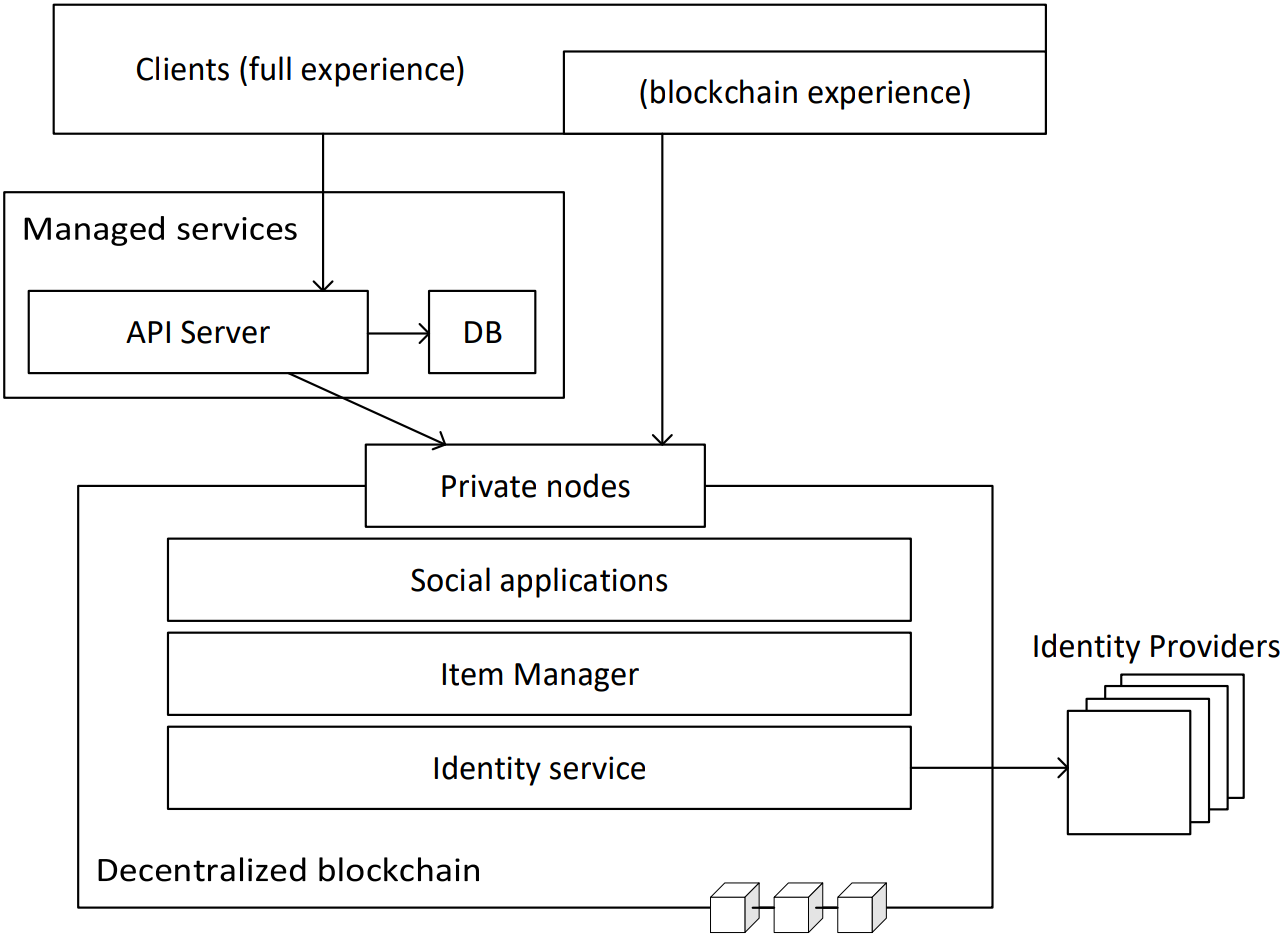
\includegraphics[scale=0.25]{img/architettura.png}
    \caption{Architettura dell'implementazione con blockchain}
    \label{fig:architettura}
\end{figure}

\subsection{Tag}
\label{tag}
Ogni tag ha un identificativo univoco che permette di identificare l'oggetto fisico o virtuale che rappresentano del quale un utente può detenere la proprietà. I tag vengono creati da un contratto, che li emette sotto forma di token non fungibili, compatibili con lo standard \emph{ERC721}. I token sono corredati da un identificativo pubblico e da eventuali chiavi private. Le chiavi private possono servire a sbloccare la proprietà del token in fase di acquisto del prodotto, oppure per la verifica dell'autenticità.
I tag possono essere di due tipi:
\begin{itemize}
    \item \emph{Personal tag}: possono essere prodotti da qualsiasi utente senza particolari requisiti e possono essere garantiti dall'utente stesso attraverso mezzi indipendenti. Sono dedicati alla catalogazione di beni personali per l'uso privato. Contengono direttamente le informazioni dell'oggetto che possono essere crittografate.
    \item \emph{Production tag}: sono destinati alla produzione di massa. Sono collegati ad un produttore e possono essere identificati come genuini se il produttore ha un certificato valido. Questi tag sono associati ad un profilo oggetto contenente le informazioni dell'oggetto stesso, che può essere modificato solamente dal produttore o dai suoi delegati. Questi tag possono essere abilitati per l'acquisto, per la verifica e possono contenere un premio di verifica.
\end{itemize}

I tag possono essere creati direttamente già attivati, oppure essere attivati successivamente dal produttore o da un venditore autorizzato. Un tag non attivo è un tag che non viene più riconosciuto dal produttore e che quindi non è più accessibile e verificabile. Se un tag è attivo può essere acquistato autonomamente da un utente finale.

I tag possono essere acquistati autonomamente da un produttore in ether tramite un contratto, oppure il produttore può rivolgersi a Digicando per pagare in altre valute. Il costo di un tag è definito arbitrariamente da bCerty, osservando il valore dell'ether nel mercato ed aggiornandolo periodicamente di conseguenza \cite{bCerty-whitepaper}.

\subsection{Verifica di un prodotto}
\label{verifica-di-un-prodotto}
Il servizio su blockchain prevede la possibilità per ogni utente di verificare l'autenticità di un prodotto tramite lo \emph{smartphone} senza la necessità di procedere con l'acquisto, ricevendo una ricompensa. Ad ogni prodotto, o lotto di prodotti, può essere infatti associato un premio, chiamato \emph{bounty}, correlato a diverse operazioni che l'utente può compiere: acquisto, verifica dell'originalità del token, scambio di oggetti tra utenti. Insieme alla conferma di originalità l'utente può ricevere delle informazioni riguardanti il prodotto. Questo processo di verifica con ricompensa permette di ottenere un controllo di anticontraffazione distribuito, senza la necessità per il produttore di organizzare esso stesso i controlli, e rende ogni utente un potenziale investigatore privato.

Ogni tag verificabile è fornito di un tag NFC leggibile e scrivibile, nel quale viene memorizzato un codice dinamico. Il codice è una chiave di crittografia privata ellittica di cui è possibile trovare la chiave pubblica corrispondente tramite la blockchain associata al tag. Se le chiavi corrispondono il tag è originale. Il sistema prevede che il codice sia aggiornato per prevenire la creazione di cloni dello stesso tag. L'aggiornamento del codice dinamico non è obbligatorio, ma il produttore può impostare dei criteri per premiare chi decide di farlo, per esempio i \emph{bounty} di verifica. Ogni operazione di verifica è tracciata sulla blockchain, fatta eccezione per le verifiche negative che innescano opzionalmente l'invio al sistema di un rapporto contenente tutti i dati necessari per comprendere l'accaduto \cite{bCerty-whitepaper}.

\paragraph{Bounty di verifica}
Ogni tag contiene un bounty di verifica, impostato dal produttore ed espresso in ether. Il bounty viene rilasciato quando il prodotto viene acquistato, distribuendolo a tutti coloro che hanno verificato l'originalità del prodotto e hanno aggiornato correttamente il codice. Il bounty viene distribuito proporzionalmente ai lassi di tempo intercorsi tra le diverse verifiche, per evitare che uno stesso utente compia diverse verifiche con diversi indirizzi per aggiudicarsi un bounty più grande.

Il produttore può prestabilire il momento di attivazione del bounty, per esempio attivandolo all'arrivo in negozio, per evitare che gli addetti al trasporto possano aggiudicarsi un bounty o che il primo verificatore si aggiudichi il bounty relativo a tutto il tempo di trasporto. In alternativa il venditore del negozio può essere incaricato dal produttore di controllare ed attivare i tag dei prodotti che riceve.

\subsection{Acquisto}
\label{acquisto}
L'acquisto viene eseguito tramite una chiave segreta stampata sul tag tramite un codice, generalmente di tipo QR. Questo codice può essere scoperto solo tramite un'azione meccanica irreversibile sul tag ed è necessario per effettuare una transazione che firma l'indirizzo dell'acquirente tramite la chiave trovata. Un contratto su blockchain verificherà poi la firma utilizzando la chiave pubblica e verificherà che l'indirizzo mostrato corrisponda al nome dell'acquirente; se corrisponde la vendita sarà autorizzata.

\subsection{Scambio e rivendita di prodotti usati}
Utilizzando un contratto specifico è possibile rivendere prodotti usati. Il contratto certifica il possesso dell'oggetto da parte del venditore e raccoglie il pagamento del compratore. Solamente quando entrambe le parti avranno completato con successo le transazioni il contratto rilascerà il credito al venditore e trasferirà il possesso al compratore. Le vendite possono essere effettuate in ether, oppure in altre valute regolate da un oracolo. 

\subsection{Memorizzazione dei dati}
Tutti i dati di grandi dimensioni e non critici dal punto di vista della privacy verranno memorizzati su IPFS o Swarm. Questi dati comprendono:
\begin{itemize}
    \item I dati multimediali.
    \item Le descrizioni testuali di prodotti, produttori, utenti ed altro.
    \item I commenti riguardanti la qualità dei prodotti e le recensioni.
\end{itemize}

I dati funzionali invece, verranno memorizzati direttamente sulla blockchain all'interno dei contratti. Questi dati comprendono, per esempio, le chiavi di sblocco dei prodotti.

Per garantire la protezione della privacy alcuni dati di servizio saranno mantenuti privati da Digicando e non saranno pubblicati sulla blockchain; questi comprendono le informazioni personali degli utenti e dei produttori, le analisi di utilizzo dell'applicazione, le informazioni riguardanti le verifiche e le letture dei tag e gli oggetti che non hanno la certificazione bCerty.

\subsection{Adozione del servizio basato su blockchain}
\label{adozione-del-servizio-basato-su-blockchain}
La transizione al servizio basato su blockchain sarà graduale e, almeno inizialmente, facoltativa, per rendere questo processo il meno problematico possibile per tutte le parti interessate. Inizialmente l'implementazione su blockchain verrà distribuita sulla \emph{testnet Ropsten} ed utilizzata unicamente per un \emph{beta testing} interno. Seguirà una fase dove le due implementazioni coesisteranno. Solamente in un secondo momento, quando il servizio su blockchain sarà completamente funzionante ed ampiamente testato, si procederà con lo spegnimento dei server non più utili al funzionamento.

\subsection{Svantaggi e considerazioni sull'utilizzo della blockchain}
\label{svantaggi-e-considerazioni}
La transizione ad un servizio basato su blockchain porta una serie di svantaggi e di problematiche da risolvere: primo fra tutti la mancanza del concetto di segretezza; ogni dato pubblicato su blockchain infatti non sarà mai completamente privato. Questo problema ha portato a varie difficoltà nell'implementazione dell'algoritmo di verifica con chiavi segrete dinamiche brevettato da Digicando, che è stato quindi modificato. Una seconda problematica, non direttamente collegata a Digicando, è la scalabilità della blockchain. Il numero di transazioni che la rete è in grado di gestire in un'unità di tempo è limitato e, attualmente, particolarmente basso. Con l'aumento degli utilizzatori della rete questo problema non può che peggiorare. In futuro si pensa di migrare il servizio su una blockchain Plasma, per risolvere questo problema. Una terza problematica infine, può essere la futura promulgazione di leggi che limitino le possibilità di utilizzo e l'adozione della tecnologia blockchain.

\newpage

      \chapter{Il problema dei ruoli}
\label{cha:problema-ruoli}
Nei seguenti capitoli viene descritto il lavoro svolto durante il tirocinio, dalla raccolta e definizione dei requisiti del sistema da sviluppare, alla sua effettiva implementazione.

Durante la fase di sviluppo dell'implementazione del servizio di Digicando su blockchain si è data priorità allo sviluppo del \emph{core} dell'applicazione. Per questo motivo alcune caratteristiche e funzioni dell'applicazione sono state inizialmente tralasciate per essere sviluppate in futuro. Una delle maggiori limitazioni dell'implementazione è l'impossibilità di gestire un brand ed il contratto principale di Digicando da più indirizzi e la mancanza di un sistema flessibile per la loro aggiunta e rimozione. Si è quindi reso necessario lo sviluppo di un sistema di gestione dei ruoli completamente su blockchain.

La gestione dei ruoli degli utenti nell'implementazione blockchain del servizio di Digicando è stata inizialmente realizzata mediante un sistema di \emph{whitelisting} di indirizzi Ethereum all'interno dei contratti stessi. Questo approccio ha comportato un irrigidimento dell'architettura al momento di eventuali aggiornamenti ed un aumento di complessità dei contratti interessati, costretti a svolgere più compiti non correlati al loro scopo.

\section{Identificazione degli operatori}
Gli operatori, cioè tutti coloro che sono in grado di eseguire determinate azioni sul sistema, saranno identificati da un servizio di identità, che si occuperà di rilasciare dei certificati non trasferibili. BCerty sarà in possesso del certificato radice, sarà in grado di emettere autorizzazioni per operare sulla piattaforma  a ciascun certificato e ne potrà emettere di nuovi. Sarà possibile incaricare altri certificatori indipendenti, che potranno operare senza la necessità di intervento da parte di bCerty. I brand avranno la possibilità di autocertificarsi. Il certificato radice sarà criptato, protetto da una chiave a firma multipla. La struttura a cascata dei certificati emessi sarà simile a quella del sistema di rilascio di certificati SSL. Ogni certificato conterrà in chiaro le informazioni pubbliche dell'ente ed i permessi attribuiti all'utente, cioè l'elenco di azioni che lo stesso sarà in grado di compiere. Un'azione possibile sarà quella di creare sottocertificati, con al più i permessi del certificato padre. Un certificato è considerato valido solamente se tutti i certificati padre, fino al certificato radice, sono validi; la revoca o la rimozione di un certificato si riperquoterà su tutti i certificati figli \cite{bCerty-whitepaper}.

\section{Requisiti}
\label{requisiti}
Si è deciso di sviluppare un nuovo contratto esterno in sostituzione del sistema di whitelisting degli indirizzi. L'approccio migliore individuato è un sistema basato su \emph{claim}, cioè una serie di attributi che gli utenti sono in grado di attribuirsi tra loro, che permettono di conferire loro particolari tipologie di privilegi. Un possibile elenco non completo di ruoli attribuibili agli utenti è:
\begin{itemize}
    \item Dipendente di Digicando autorizzato a certificare nuovi brand.
    \item Produttore di tag per un brand, in grado di emettere nuovi oggetti unici.
    \item Venditore autorizzato per un determinato prodotto.
\end{itemize}

\noindent
I requisiti e le caratteristiche importanti individuati per il sistema insieme all'azienda sono:
\begin{itemize}
    \item Il sistema di gestione dei ruoli deve essere sviluppato per lavorare interamente sulla blockchain Ethereum.
    \item Il sistema deve essere dinamico sulla creazione di nuovi ruoli: i ruoli ammessi e gestiti dal sistema non devono essere limitati ad un insieme fisso e non deve essere necessario sviluppare e distribuire un nuovo contratto ogni volta si renda necessario supportare un nuovo ruolo.
    \item I ruoli devono poter essere gestiti in maniera gerarchica a cascata: un utente con un ruolo può avere il permesso di emettere dei ruoli a sua volta, che saranno considerati validi finchè il suo ruolo sarà valido.
    \item Ogni operatore potrà avere differenti privilegi, compreso quello di nominare dei collaboratori con privilegi uguali o inferiori ai suoi.
    \item Ogni indirizzo deve poter emettere un ruolo ad un qualsiasi altro indirizzo. Il sistema non avrà il compito di controllare l'emissione dei ruoli, ma solo di memorizzarla e gestirla. Il sistema deve inoltre fornire delle funzioni di verifica della validità di singoli ruoli o di catene di ruoli. Dare un significato ed un valore ai ruoli sarà compito delle applicazioni che utilizzeranno il sistema.
    \item Gli operatori devono poter agire in autonomia, nei limiti delle possibilità a loro attribuite.
    \item Un utente deve poter ricevere lo stesso ruolo da più garanti.
\end{itemize}

      \chapter{Implementazione}
\label{cha:implementazione}
In questo Capitolo viene descritta la fase di implementazione del sistema, che comprende lo sviluppo in accordo ai requisiti individuati, l'integrazione con il sistema implementato da Digicando ed il testing.

\section{Tecnologie utilizzate}
Per lo sviluppo del sistema sono state utilizzate le migliori tecnologie disponibili per lo sviluppo di smart contracts su blockchain Ethereum. Tutte le tecnologie utilizzate sono open-source, seguendo la filosofia della blockchain Ethereum, e sviluppate da una community di sviluppatori. Le principali sono:
\begin{itemize}
    \item \emph{Linguaggio di programmazione Solidity}: un linguaggio di programmazione ad alto livello orientato agli oggetti per lo sviluppo di smart contracts \cite{solidity-documentation}.
    \item \emph{Truffle}: un ambiente di sviluppo, un framework per il testing ed un insieme di risorse per la blockchain Ethereum \cite{trufflesuite}.
    \item \emph{Ganache}: uno strumento per creare blockchain Ethereum personali, utilizzabili per pubblicare contratti durante il loro sviluppo e condurre dei test \cite{trufflesuite}.
\end{itemize}

\section{I contratti}
\label{sec:contratti}
Il sistema di gestione dei ruoli è stato sviluppato nel linguaggio di programmazione ad alto livello per blockchain Ethereum \emph{Solidity}. Il sistema sviluppato è composto da due contratti:
\begin{itemize}
    \item \emph{ClaimsRegister}: memorizza i ruoli emessi.
    \item \emph{ClaimsManagement}: permette di gestire delle strutture organizzative dei ruoli gerarchiche e complesse.
\end{itemize}

\subsection{ClaimsRegister}
\label{claims-register}
Funge da registro per la memorizzazione di ruoli, chiamati \emph{claim}, con associato un valore da un emettitore ad un ricevitore. Si è scelto di utilizzare la parola \emph{claim} e non \emph{role} per mantenere una maggiore genericità e rendere il sistema più versatile. In pratica, una claim è una tupla formata da un emettitore, un ricevitore, la chiave della claim ed il relativo valore. Ogni indirizzo può emettere ruoli ad ogni indirizzo, infatti non è presente alcuna logica di controllo sui ruoli e la loro emissione ed il registro non conosce il significato dei ruoli. Spetterà alle applicazioni che utilizzeranno il registro implementare i meccanismi di controllo e dare un significato ai ruoli. Il contratto implementa due funzioni, per l'aggiunta e la rimozione dei ruoli.

Questo contratto, da solo, permette di gestire delle strutture organizzative dei ruoli ad un livello dove ogni utente ha gli stessi diritti degli altri e può rimuovere ed aggiungere utenti.

\paragraph{Registro di claim}
Il registro è un \texttt{mapping}, cioè una \emph{tabella hash} nel linguaggio Solidity, che memorizza un valore associato a tre chiavi.

\noindent
\begin{lstlisting}[language=Solidity]
    // emitter => receiver => claim => value
    mapping(address => mapping(address => mapping(bytes32 => bytes32))) public registry;
\end{lstlisting}

Le chiavi della tabella sono, in ordine:
\begin{itemize}
    \item \emph{Emitter}: è l'indirizzo Ethereum che emette il ruolo.
    \item \emph{Receiver}: è l'indirizzo Ethereum che riceve il ruolo.
    \item \emph{Claim}: è un array di 32 bytes che rappresenta la chiave di un ruolo. Un possibile metodo per l'identificazione di una chiave adeguata per un ruolo è calcolare l'hash di una stringa che descriva il ruolo.
\end{itemize}
Il valore \emph{value} associato alle tre chiavi è nuovamente un array di 32 bytes e rende il registro molto flessibile e versatile quando utilizzato da un'applicazione. Il valore, infatti, può essere utilizzato di base per memorizzare un valore booleano, ma un'applicazione può utilizzarlo per memorizzare informazioni con significati più ampi.

\paragraph{Metodi}
Il contratto implementa due metodi: uno per l'aggiunta e uno per la rimozione di claim.

\noindent
\begin{lstlisting}[language=Solidity]
    function setClaim(address receiver, bytes32 claim, bytes32 value)
        public
    {
        registry[msg.sender][receiver][claim] = value;
    }
\end{lstlisting}
Emette una claim dall'indirizzo che chiama la funzione ad un ricevitore specificato.

\noindent
\begin{lstlisting}[language=Solidity]
    function removeClaim(address receiver, bytes32 claim)
        public
    {
        delete(registry[msg.sender][receiver][claim]);
    }
\end{lstlisting}
Rimuove una claim precedentemente emessa dall'indirizzo che chiama la funzione ad un ricevitore specificato.

L'utilizzo di \texttt{msg.sender} nell'identificazione dell'emettitore nei due metodi assicura che solamente il possessore della chiave privata associata ad un indirizzo possa emettere e rimuovere claim con tale indirizzo.

\subsection{ClaimsManagement}
\label{claims-management}
Questo contratto implementa una funzione per il controllo della validità di catene di claim. Una catena di claim è valida solamente se ogni claim al suo interno esiste nel registro e se valgono le seguenti regole:
\begin{itemize}
    \item La prima claim è emessa da un indirizzo, chiamato \emph{root}, ad un ricevitore.
    \item Ogni claim successiva è emessa dal ricevitore della precedente.
\end{itemize}

Il contratto non memorizza le catene di claim, ma permette solamente il controllo della loro validità. Spetta alle applicazioni mantenere con delle strutture dati apposite. Il sistema permette la creazione ed il mantenimento di strutture organizzative gerarchiche complesse e ammette la presenza di più indirizzi \emph{radice} e la possibilità per un indirizzo di ricevere la stessa claim da più emettitori.

\begin{figure}[ht!]
    \centering
    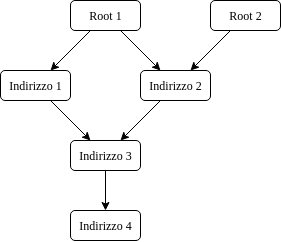
\includegraphics[scale=0.75]{img/gerarchia.png}
    \caption{Esempio di gerarchia complessa}
    \label{fig:gerarchia}
\end{figure}

\paragraph{Il metodo}
La funzione riceve in ingresso tre vettori:
\begin{itemize}
    \item \emph{chain}: la catena di utenti, ordinati dall'ultimo ricevitore alla root.
    \item \emph{claims}: la catena delle chiavi delle claim, dall'ultima alla prima.
    \item \emph{values}: la catena dei valori delle claim, dall'ultimo al primo.
\end{itemize}

La funzione effettua, per prima cosa, dei controlli sulle lunghezze dei vettori passati come parametri. Se i controlli vengono rispettati, la funzione procede a ciclare e verificare le claim della catena. Se una claim non risulta valida nel registro, la funzione ritorna \texttt{false}, se tutte le claim sono verificate ritorna \texttt{true}.

\noindent
\begin{lstlisting}[language=Solidity]
    function checkClaims(address[] memory chain, bytes32[] memory claims, bytes32[] memory values)
        public
        view
        returns (bool)
    {
        require(claims.length == chain.length - 1, "The length of the arrays is wrong");
        require(claims.length == values.length, "The length of the arrays is wrong");
    
        for(uint i = 0; i < chain.length - 1; i++){
            if(register.registry(chain[i + 1], chain[i], claims[i]) != values[i]) {
                return false;
            }
        }
    
        return true;
    }
\end{lstlisting}

\section{Integrazione}
Il processo di integrazione del nuovo sistema di gestione dei ruoli è proseguita per fasi. Per prima cosa è stata studiata l'implementazione attuale ed è stato modellato un diagramma delle classi per avere una vista più chiara del sistema nel suo complesso. Lo studio dell'implementazione ha avuto come obiettivo l'individuazione dei contratti che facevano uso del sistema di \emph{whitelisting}. Infine, ogni riferimento al vecchio sistema è stato rimosso e sostituito con la nuova soluzione sviluppata. Il sistema integrato è stato testato approfonditamente, mediante l'utilizzo di test automatici e pubblicandolo in una blockchain privata.

\section{Utilizzi}
L'attuale implementazione nella quale è stato integrato il sistema di gestione dei ruoli ne utilizza soltanto le funzioni di base, per mantenere e gestire un'organizzazione a singolo livello. Il sistema di gestione dei ruoli viene attualmente utilizzato per gestire i \emph{manager}, cioè coloro che hanno il permesso di effettuare azioni avanzate, di due contratti:
\begin{itemize}
    \item \emph{BcertyHub}: questo è il contratto principale della nuova implementazione su blockchain del servizio di Digicando. Permette al personale Digicando di registrare nuovi produttori e verificarli, di gestire delle configurazioni avanzate e di aggiornare il costo dei tag. 
    \item \emph{BcertyProducer}: è il contratto che permette ad un produttore ed i suoi collaboratori di gestire le proprie informazioni, di creare ed abilitare dei tag e di gestire i propri prodotti.
\end{itemize}

\subsection{Management}
Per gestire i manager è stato sviluppato un nuovo contratto, chiamato \emph{Management}, che utilizza le funzioni di base del registro di claim. Per utilizzare questo contratto è necessario ereditarlo come segue:
\noindent
\begin{lstlisting}[language=Solidity]
    contract Example is Management {}
\end{lstlisting}

Il contratto implementa due funzioni, per l'aggiunta e la rimozione di un manager. All'aggiunta di un manager, viene emessa una claim così formata:
\begin{itemize}
    \item \emph{Emitter}: l'indirizzo stesso del contratto Management.
    \item \emph{Receiver}: l'indirizzo del nuovo manager.
    \item \emph{Claim}: una costante che contiene l'hash della stringa \emph{MANAGER}, calcolato mediante la funzione di hashing \texttt{keccak256()}.
    \item \emph{Value}: una costante che contiene l'hash della stringa \emph{TRUE}.
\end{itemize}

\noindent
\begin{lstlisting}[language=Solidity]
    bytes32 private MANAGER = keccak256("MANAGER");
    bytes32 private TRUE = keccak256("TRUE");

    function setManager(address newManager)
        public
        onlyManager
    {
        claimsRegister.setClaim(newManager, MANAGER, TRUE);
    }

    function removeManager(address manager)
        public
        onlyManager
    {
        claimsRegister.removeClaim(manager, MANAGER);
    }
\end{lstlisting}

Queste due azioni possono essere compiute solamente da un manager; questo controllo viene effettuato dal modificatore \texttt{onlyManager}. Un modificatore è uno speciale tipo di funzione che viene applicato ad altre funzioni aggiungendone il nome nella dichiarazione. I modificatori sono utilizzati per creare delle condizioni che si applicano a diverse funzioni in un contratto, in modo da non dover riscrivere lo stesso codice molteplici volte.

\noindent
\begin{lstlisting}[language=Solidity]
    /**
     * @dev Throws if called by any account other than a manager.
     */
    modifier onlyManager()
    {
        require(isManager(), "You are not a manager");
        _;
    }
\end{lstlisting}

Il modificatore controlla che l'indirizzo che sta provando ad eseguire l'azione sia un manager, servendosi della funzione \texttt{isManager()}, che legge il registro per verificare la presenza della claim e ritorna \texttt{true} in caso positivo e \texttt{false} altrimenti.

\noindent
\begin{lstlisting}[language=Solidity]
    /*
     * @return true if `msg.sender` is a manager of the contract.
     */
    function isManager()
        public view
        returns (bool)
    {
        return claimsRegister.registry(
            address(this),
            msg.sender,
            MANAGER) == TRUE;
    }
\end{lstlisting}

\section{Testing}
La suite \emph{truffle} permette di scrivere dei test automatici in \emph{JavaScript} per verificare il funzionamento dei contratti dal mondo esterno, simulando un'applicazione. Per effettuare i test è necessario creare una blockchain privata con \emph{ganache}, su cui i contratti verranno pubblicati ed eseguiti. Per ogni contratto è stato sviluppato un relativo test. Alla creazione della blockchain privata ganache mette a disposizione dieci account, che possono essere utilizzati nei test tramite un vettore chiamato \texttt{accounts}.

\subsection{ClaimsRegister}
Il file di test per il contratto \emph{ClaimsRegister} contiene due semplici \emph{unit-test}, relativi alle due funzioni del contratto. Il primo test emette una nuova claim dall'account \texttt{0} all'account \texttt{1} e subito ne verifica l'effettiva emissione. Il secondo test rimuove la claim precedentemente emessa e successivamente verifica che non sia effettivamente più presente nel registro.

\noindent
\begin{minipage}{\linewidth}
\begin{lstlisting}[language=JavaScript]
const testClaim = web3.utils.keccak256("TEST_CLAIM");
const testValue = web3.utils.keccak256("TEST_VALUE");

const ClaimsRegister = artifacts.require("ClaimsRegister");

contract("ClaimsRegister", accounts => {
    it("Set claim", async () => {
        const instance = await ClaimsRegister.deployed();

        await instance.setClaim(accounts[1], testClaim, testValue, {
            from: accounts[0]
        });

        var value = await instance.registry.call(accounts[0], accounts[1], testClaim);

        assert.equal(value, testValue, "The value of the claim was not set correctly");
    });

    it("Remove claim", async () => {
        const instance = await ClaimsRegister.deployed();

        await instance.removeClaim(accounts[1], testClaim, {
            from: accounts[0]
        });

        var value = await instance.registry.call(accounts[0], accounts[1], testClaim);

        assert.equal(value, 0, "The claim was not removed correctly");
    });
});
\end{lstlisting}
\end{minipage}

\subsection{ClaimsManagement}
Il file di test relativo al contratto \emph{ClaimsManagement} consiste di una parte di \emph{setup} e di uno \emph{unit-test} per la funzione di controllo della validità di una catena di claim. Durante la fase di setup vengono emesse due claim, che vanno a formare una catena. La prima claim viene emessa dall'account \texttt{0} all'account \texttt{1} e la seconda dall'account \texttt{1} all'account \texttt{0}. Lo unit-test, invece, chiama la funzione passando per parametro i vettori contenenti le componenti della catena di claim e ne verifica la validità.

\noindent
\begin{minipage}{\linewidth}
\begin{lstlisting}[language=JavaScript]
const testClaim = web3.utils.keccak256("TEST_CLAIM");
const testValue = web3.utils.keccak256("TEST_VALUE");

const ClaimsManagement = artifacts.require("ClaimsManagement");
const ClaimsRegister = artifacts.require("ClaimsRegister");

contract("ClaimsManagement", accounts => {
    it("Setup...", async () => {
        const instance = await ClaimsRegister.deployed();

        await instance.setClaim(accounts[1], testClaim, testValue, {
            from: accounts[0]
        });

        await instance.setClaim(accounts[2], testClaim, testValue, {
            from: accounts[1]
        });
    });

    it("Check claims", async () => {
        const instance = await ClaimsManagement.deployed();

        var chain = new Array();
        chain.push(accounts[2], accounts[1], accounts[0]);

        var claims = new Array();
        claims.push(testClaim, testClaim);

        var values = new Array();
        values.push(testValue, testValue);

        var valid = await instance.checkClaims.call(chain, claims, values);

        assert.equal(valid, true, "The claims are not valid");
    }); 
});
\end{lstlisting}
\end{minipage}

\begin{figure}[ht!]
    \centering
    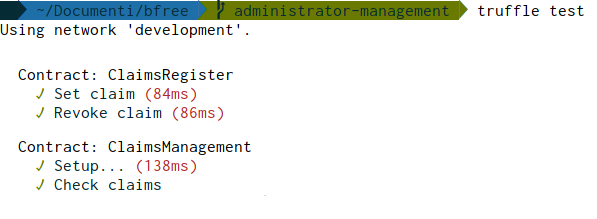
\includegraphics[scale=0.5]{img/test.png}
    \caption{L'esito positivo dei test automatici}
    \label{fig:test}
\end{figure}

\newpage

      \chapter{Conclusioni}
\label{cha:conclusioni}
Gli obiettivi principali del tirocinio erano comprendere i principi alla base di una blockchain ed i relativi strumenti di programmazione, sviluppare capacità di analisi, di progettazione software e di lavorare in team. Terminato il tirocinio gli obiettivi possono essere considerati raggiunti. In particolare, sono state acquisite le competenze per lo sviluppo di applicazioni basate sulla blockchain.

I requisiti individuati dall'azienda per il sistema sono stati soddisfatti ed il sistema sviluppato si è integrato correttamente con le parti del servizio già implementate risolvendo il problema dei ruoli, descritto nel capitolo \ref{cha:problema-ruoli}. La soluzione sviluppata permette di gestire i contratti da molteplici indirizzi, senza la necessità di avere un indirizzo condiviso da tutti gli utenti autorizzati. Questo porta ad una maggiore sicurezza del sistema, permettendo in caso di necessità di revocare l'autorizzazione a determinati utenti.
Il contratto \emph{Management} presenta una criticità nota, dovuta al fatto che durante lo sviluppo si è data priorità alla semplicità, piuttosto che alle funzionalità. Questa criticità permette ad un utente autorizzato come manager che diventi malevolo di rimuovere tutti gli altri manager, ottenendo il controllo esclusivo del contratto.

L'implementazione blockchain del servizio di Digicando verrà resa open-source in futuro, quindi chiunque avesse la necessità di un sistema di gestione dei ruoli su blockchain Ethereum potrà adottare il sistema descritto in questa tesi ed integrarlo nel proprio progetto.

    \endgroup


    % bibliografia in formato bibtex
    %
    % aggiunta del capitolo nell'indice
    \addcontentsline{toc}{chapter}{Bibliografia}
    % stile con ordinamento alfabetico in funzione degli autori
    \bibliographystyle{plain}
    \bibliography{biblio}
%%%%%%%%%%%%%%%%%%%%%%%%%%%%%%%%%%%%%%%%%%%%%%%%%%%%%%%%%%%%%%%%%%%%%%%%%%
%%%%%%%%%%%%%%%%%%%%%%%%%%%%%%%%%%%%%%%%%%%%%%%%%%%%%%%%%%%%%%%%%%%%%%%%%%
%% Nota
%%%%%%%%%%%%%%%%%%%%%%%%%%%%%%%%%%%%%%%%%%%%%%%%%%%%%%%%%%%%%%%%%%%%%%%%%%
%% Nella bibliografia devono essere riportati tutte le fonti consultate 
%% per lo svolgimento della tesi. La bibliografia deve essere redatta 
%% in ordine alfabetico sul cognome del primo autore. 
%% 
%% La forma della citazione bibliografica va inserita secondo la fonte utilizzata:
%% 
%% LIBRI
%% Cognome e iniziale del nome autore/autori, la data di edizione, titolo, casa editrice, eventuale numero dell’edizione. 
%% 
%% ARTICOLI DI RIVISTA
%% Cognome e iniziale del nome autore/autori, titolo articolo, titolo rivista, volume, numero, numero di pagine.
%% 
%% ARTICOLI DI CONFERENZA
%% Cognome e iniziale del nome autore/autori (anno), titolo articolo, titolo conferenza, luogo della conferenza (città e paese), date della conferenza, numero di pagine. 
%% 
%% SITOGRAFIA
%% La sitografia contiene un elenco di indirizzi Web consultati e disposti in ordine alfabetico. 
%% E’ necessario:
%%   Copiare la URL (l’indirizzo web) specifica della pagina consultata
%%   Se disponibile, indicare il cognome e nome dell’autore, il titolo ed eventuale sottotitolo del testo
%%   Se disponibile, inserire la data di ultima consultazione della risorsa (gg/mm/aaaa).    
%%%%%%%%%%%%%%%%%%%%%%%%%%%%%%%%%%%%%%%%%%%%%%%%%%%%%%%%%%%%%%%%%%%%%%%%%%
%%%%%%%%%%%%%%%%%%%%%%%%%%%%%%%%%%%%%%%%%%%%%%%%%%%%%%%%%%%%%%%%%%%%%%%%%%
    

    %\titleformat{\chapter}
    %    {\normalfont\Huge\bfseries}{Allegato \thechapter}{1em}{}
    % sezione Allegati - opzionale
    %\appendix
    %\input{allegati}

\end{document}